
\documentclass[]{report}

\voffset=-1.5cm
\oddsidemargin=0.0cm
\textwidth = 480pt

\usepackage{framed}
\usepackage{subfiles}
\usepackage{graphics}
\usepackage{newlfont}
\usepackage{eurosym}
\usepackage{amsmath,amsthm,amsfonts}
\usepackage{amsmath}
\usepackage{color}
\usepackage{amssymb}
\usepackage{multicol}
\usepackage[dvipsnames]{xcolor}
\usepackage{graphicx}
\begin{document}

% BIVARIATE
%-------------------------------------------------%

%---------------------------------------------------------------------%

\section{Bivariate Data}
\begin{itemize}
	\item Very often we are interested in the relationship between two
	variables.
	\item For example we might be interested in the relationship between
	unemployment and inflation.
	\item The investigation of a relationship between two variables
	begins with an attempt to discover the approximate form of the
	relationship by graphing the data using a scatter plot.
\end{itemize}	
\subsection*{Terminology}
\begin{itemize}
	\item Univariate statistics describes statistics related to one variables.
	\item Bivariate statistics describes statistics related to two variables $X$ and $Y$.
	\item Multivariate statistics describes statistics related to multiple variables (not part of course).
\end{itemize}



%---------------------------------------------------------------------%

\subsection*{Variables in Bivariate Data}
\begin{itemize}
	\item  A scatter plot is a two-dimensional plot showing the (x,y) value for each
	observation.
	
	\item  Using these plots, we can quickly determine whether there is
	any pronounced relationship and if so, whether the relationship may be
	treated as approximately \textbf{linear}.\\
	\begin{itemize}
		\item Response variable Y (dependent variable).\\
		\item Predictor variable X (independent variable).
	\end{itemize}
	\item A response variable is the variable whose variation we wish to explain.
	\item The predictor variable is a variable used to explain the variation in the
	response variable.
\end{itemize}
%---------------------------------------------------------------------%

\section{Scatterplots}
Scatterplots are used to visualize the relationship between two continuous variables. The position of each point on the plot indicates the meaurement by both variables. Scatterplots are useful for determining the possible relationship between the variables.

\begin{itemize}
	\item The first step in determining the relationship between two
	variables is to draw a scatter plot.
	\item After establishing that a linear relationship exists between the
	two variables X and Y, we need to measure the strength of this
	relationship.
	\item In order to do this, we need some measure of the association
	or relationship between the two variables.
	\item There are several ways of doing this - the most common
	measure is the Pearson product moment correlation
	coefficient usually known as the correlation coefficient.
	
\end{itemize}



%-------------------------------------------------%
% R Code
%
% X = c(10, 15, 20, 25, 30, 35, 40)
% Y = c(11, 19, 34, 52, 58, 81, 109)
% plot(X,Y,pch=18,col="red",font.lab=2,main="Scatter Plot of X and Y")
% cor(X,Y) =0.9830478

%-------------------------------------------------%

\subsection{Scatter-plots}
Subsequent Slides
\begin{itemize}
	\item Relatively strong positive relationship (as height increases
	weight on average increases), reasonably linear.
	\item No relationship/weak negative relationship
	\item Negative, very strong, non-linear relationship.
	\item Non-linear relationship.
\end{itemize}


\subsection*{Inspecting Scatter Plots (1) }
\begin{figure}[h!]
	% Requires \usepackage{graphicx}
	\includegraphics[scale=0.7]{images/11BPlot1.jpg}\\
\end{figure}
Relatively strong positive relationship (as height increases
weight on average increases), reasonably linear.

\subsection*{Inspecting Scatter Plots (2) }
\begin{figure}[h!]
	% Requires \usepackage{graphicx}
	\includegraphics[scale=0.7]{images/11BPlot2.jpg}\\
\end{figure}

No relationship (at a stretch, a very weak negative relationship).

\subsection*{Inspecting Scatter Plots (3) }
\begin{figure}[h!]
	% Requires \usepackage{graphicx}
	\includegraphics[scale=0.7]{images/11BPlot3.jpg}\\
	
\end{figure}

Negative, very strong, non-linear relationship



\subsection*{Inspecting Scatter Plots (4) }
\begin{figure}[h!]
	% Requires \usepackage{graphicx}
	\includegraphics[scale=0.7]{images/11BPlot4.jpg}\\
\end{figure}
Non- Linear Relationship


\subsection{Detecting Outliers}

Be mindful that the corration may be spurious. That is to say : The scatterplot indicates a relationship that does not really exist. Rather the points align in a linear manner on the scatterplot by chance. Special consideration should go into designing a scientific experiment to avoid such problems, including that there is a suitably large sample size. As the sample size gets less likely spurious correlation is less likely. 


\subsection{Detecting Outliers}
\begin{itemize}
	\item A scatter plot may also be used to find outliers. These are
	observations that do not fit the pattern of the remaining data.
	\item Outliers may be due to mistakes in recording data.
	\item To check the sensitivity of analysis to such outliers, analysis should
	be carried out both with and without these outliers.
\end{itemize}

%-------------------------------------------------%
% R Code
%
% X = c(10, 15, 20, 25, 30, 35, 40)
% Y = c(11, 19, 34, 52, 58, 81, 109)
% plot(X,Y,pch=18,col="red",font.lab=2,main="Scatter Plot of X and Y")
% cor(X,Y) =0.9830478


%-------------------------------------------------%
\newpage
\subsection{Covariance}
Covariance is a strength of the measure of the linear relationship between two variables.
\[ cov(x,Y) = \]


%-------------------------------------------------%


\subsection{Scatter plots}

The first part of the question will require the drawing of a scatter plot. 
When doing do, remember to label the axes, and to put in the relevant units. (I.e. Metres, Degrees, Hours etc)

The Explanatory variable is on the X-axis and the Response variable is on the Y Axis.

A Trend line will be useful in demonstrating what type of relationship exists between the response variable and the explanatory variable.

\begin{enumerate}
	\item There are five possible plot types
	\item Strong positive linear relationship 
	\item Weak positive linear relationship
	\item Strong negative linear relationship
	\item Weak negative linear relationship
	\item No Relationship
\end{enumerate}
In the strong case – the points of the graph correspond to the trend line quite closely, whereas in the weak case they don’t.
In the positive case the response values Y increase as the explanatory values X increases. In the negative case the response values Y decrease as the explanatory values X increases. 


%-------------------------------------------------------------%



Part II 	Correlation


This Correlation value indicates weak positive linear relationship between temperatures and year.


%-------------------------------------------------%



	






\begin{center}
\begin{figure}[h!]
	% Requires \usepackage{graphicx}
	\includegraphics[scale=0.5]{images/11BPlot1.jpg} \includegraphics[scale=0.6]{images/11BPlot2.jpg}\\
	\includegraphics[scale=0.5]{images/11BPlot3.jpg} \includegraphics[scale=0.5]{images/11BPlot4.jpg}\\
	
	
\end{figure}
\end{center}
\textbf{Inspecting Scatter Plots (1) }

Relatively strong positive relationship (as height increases
weight on average increases), reasonably linear.



\begin{figure}[h!]
	% Requires \usepackage{graphicx}
	
\end{figure}

No relationship (at a stretch, a very weak negative relationship).

%\begin{figure}[h!]
%	% Requires \usepackage{graphicx}
%	\includegraphics[scale=0.5]{11BPlot1.jpg} \includegraphics[scale=0.6]{11BPlot2.jpg}\\
%	\includegraphics[scale=0.5]{11BPlot3.jpg} \includegraphics[scale=0.5]{11BPlot4.jpg}\\
%	
%	
%\end{figure}

Negative, very strong, non-linear relationship








%---------------------------------------------------------------------%

\textbf{Correlation Coefficient : Summations}

\begin{figure}
	% Requires \usepackage{graphicx}
	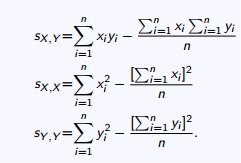
\includegraphics[scale=0.7]{images/11Bpearson.jpg}\\
	\caption{Summations}\label{11bpear}
\end{figure}


\begin{figure}
	% Requires \usepackage{graphicx}
	\includegraphics[scale=0.7]{images/11BPlot1.jpg}\\
	
\end{figure}
$r_{xy} = 0.87$ Strong Positive Linear Relationship



\begin{figure}
	% Requires \usepackage{graphicx}
	\includegraphics[scale=0.7]{images/11BPlot2.jpg}\\
	
\end{figure}

$r_{xy} = -0.258$ (Almost) No Relationship


\begin{figure}
	% Requires \usepackage{graphicx}
	\includegraphics[scale=0.7]{images/11BPlot3.jpg}\\
	
\end{figure}

$r_{xy} = -0.954$ Strong, though clearly non-linear



\textbf{Correlation Coefficients (4) }
\begin{figure}
	% Requires \usepackage{graphicx}
	\includegraphics[scale=0.7]{images/11BPlot4.jpg}\\
	
\end{figure}
$r_{xy} =  -0.051$ (although there is a very strong
relationship)

%---------------------------------------------------------------------%
\newpage
\section{Regression}
A statistical measure that attempts to determine the strength of the relationship between one dependent variable
(usually denoted by Y) and a series of other changing variables (known as independent variables).

Regression takes a group of random variables, thought to be predicting Y, and tries to find a mathematical relationship between them. This relationship is typically in the form of a straight line (linear regression) that best approximates all the individual data points.








\begin{itemize}
	\item  Two variables that have no linear relationship have a correlation close to zero. 
	
	\item Scatterplots are a useful way of determing the likely relationship between two variables. 
	
	\item The pearson correlation coefficient is most commonly used estimate for correlation. Other types of correlation are tbe Spearman Rho correlation and the Kendal Tau. 
	
	\item  These are not not part of this course,but it is important to know that they exist. 
\end{itemize}


%-----------------------------------------------------%


The Pearson correlation estimate, which us based on sample data, is denoted r (although related metrics use capital R) .This measure is used as an estimate for the Population correlation, denoted by the greek letter Rho. 
The estimate is computed using summation identities (See the formulae ). 

Equivalently it can be computed using the  Sums of Squares Identities that are used to compute covariance and standard deviation \[\mbox{INSERT FORMULA}\] .

\subsection{Example}
determine the correlation estimate for the Spend V Impressions data.  




\subsection{Outliers}
Outliers can greatly influence the computed value of an estimate.
Correlation is closely related to Simple linear regression models, in that both are concerned with the linear relationship between variables. However Linear Regression has a different emphasis.

Simple Linear Regression describes one independent variable (IV) and the response of the dependent variable (DV). 




\subsection{Correlation and Causality }
\begin{itemize}
	\item Implicit is simple linear regression is the notion of causality. The dependent variable changes as the independent variable changes. The converse is not true.
	
\item some examples : hot temperature / ice cream example.
	
\item Correlation is not concerned with causality at all, hence the often used expression "causation does not imply causality".
	
\end{itemize}





\subsection{Regression Analysis: Example}
In a study of a wholesaler’s distribution costs, undertaken with a view to controlling cost, the volume of goods handled and the overall costs were recorded for one month in each of ten depots in a distribution network. The results are presented in the following table. Perform a regression analysis of the cost (Y ) on the volume (X).

\begin{center}
	
	\begin{tabular}{|c|c|c|}\hline
		&  Volume (X)   &  Costs (Y) \\ \hline
		1     &     48     &   20 \\
		2     &    57      &   22 \\
		3     &    49      &   19 \\
		4     &    45      &   18 \\
		5     &    50      &   20 \\
		6     &    62      &   24 \\
		7     &    58      &   21 \\
		8     &    55      &   21 \\
		9     &    38      &   15 \\
		10    &    51      &  20 \\ \hline
	\end{tabular}
\end{center}
%X=c(48,57,49,45,50,62,58,55,38,51)
%Y=c(20,22,19,18,20,24,21,21,15,20)








%-----------------------------------------------------------------------%

% # cor(X,Y) = 0.92
% X = c(19.5, 23.84, 15.34, 23.37, 13.82, 16.48, 16.15, 16.76, 17.49, 17.4, 25.42, 29.29)
% Y = c(24.41, 26.91, 24.33, 25.5, 22.84, 24.35, 23.59, 23.98, 24.65, 22.56, 26.78, 28.68)
%
% X=c(20.88, 11.72, 21.39, 15.97, 19.58, 17.2, 16.47, 20.04, 16.7, 22.23, 24.87, 23.94)
% Y=c(24.18, 27.28, 23.79, 24.84, 24.36, 24.75, 25.93, 24.76, 25.26, 22.97, 23.71, 22.75)

%-----------------------------------------------------------------------%

\section{Scatterplots}





Strength of a linear relationship between $X$ and $Y$

\begin{framed}
	\begin{verbatim}
	M=1000
	CorrData=numeric(M)
	for (i in 1:M)
	{
	CorrData[i] = cor(rnorm(10),rnorm(10))
	}
	\end{verbatim}
\end{framed}



Part 2 Correlation
This requires a simple calculation based in values given and the relevant formula.



	
\end{document}
